\documentclass[11pt, a4paper, titlepage]{article}
\usepackage[left=2cm, right=2cm, top=2cm, bottom=2cm]{geometry}
\usepackage[style=authoryear,backend=bibtex]{biblatex}
\usepackage{graphicx}
\bibliography{Proposal}

\begin{document}

\begin{titlepage} % Suppresses headers and footers on the title page
	
	\centering % Centre everything on the title page
	
	\scshape % Use small caps for all text on the title page
	
	\vspace*{\baselineskip} % White space at the top of the page
	
	%------------------------------------------------
	
	%	Title
	
	%------------------------------------------------
	
	\rule{\textwidth}{1.6pt}\vspace*{-\baselineskip}\vspace*{2pt} % Thick horizontal rule
	
	\rule{\textwidth}{0.4pt} % Thin horizontal rule
	
	\vspace{0.75\baselineskip} % Whitespace above the title
	
	{\LARGE Factors influencing the amphibian mycobiome, with a focus on known and unknown chytrids \\} % Title
	
	\vspace{0.75\baselineskip} % Whitespace below the title

	\rule{\textwidth}{0.4pt}\vspace*{-\baselineskip}\vspace{3.2pt} % Thin horizontal rule
	
	\rule{\textwidth}{1.6pt} % Thick horizontal rule
	
	\vspace{2\baselineskip} % Whitespace after the title block
	
	%------------------------------------------------
	
	%	Subtitle
	
	%------------------------------------------------
	
	MRes Project Proposal % Subtitle or further description
	
	\vspace*{3\baselineskip} % Whitespace under the subtitle
	
	%------------------------------------------------
	
	%	Editor(s)
	
	%------------------------------------------------
	
	\vspace{0.5\baselineskip} % Whitespace before the editors
	
	{\scshape\Large Lucy Goodyear \\
		Imperial College London} % Editor list
	
	\vspace{0.5\baselineskip} % Whitespace below the editor list
	
		\vspace{0.5\baselineskip} % Whitespace before the editors
	
	{\scshape\Large Supervisor: Matthew Fisher} % Editor list

	\textit{matthew.fisher@imperial.ac.uk}
	
\end{titlepage}

%\title{Factors influencing amphibian mycobiome, with a focus on known and unknown chytrids}
%\author{Lucy Goodyear}
%\date{\parbox{\linewidth}{\centering%
%		\bigskip
%		Supervisor: Professor Matthew Fisher %\endgraf \bigskip
%		matthew.fisher@imperial.ac.uk \endgraf \bigskip
%		Dept.\ of Public Health \endgraf \bigskip
%		Imperial College}}


	%\maketitle

\subsection*{Keywords}
Chytrid; Amphibian; Mycobiome; DNA barcoding; Fungus; Novel lineages

\section{Introduction}

Chytridiomycosis, caused by the amphibian chytrid fungus \textit{Batrachochytrium dendrobatidis} (\textit{Bd}), has been causing extirpations and extinctions in frogs over the past decades, with a presumed 90 extinctions, and has been linked to the decline of over 500 more species \parencite{Scheele2019}. \textit{Batrachochytrium Salamandrivorans} (\textit{BSal}), another chytrid fungus, is a more recently emerged, highly virulent pathogen related to \textit{Bd} \parencite{Martel2013}. \textit{BSal} was discovered over 20 years after \textit{Bd} and is the identified cause of declines in fire salamanders in Europe. Given the discovery of \textit{BSal} and the prediction that more than 92\% of fungal species are yet to be described, it is thought that there may be other undiscovered chytrids \parencite{hawksworth2017fungal}. Of these novel chytrids, it is highly likely that some have the potential to cause another epizootic in the future, while others may cause the competitive exclusion of \textit{Bd} and/or \textit{BSal}.

\noindent In the past few years, there has been an increase in research on the amphibian skin microbiome, for example that by \parencite{Bates2018} and \parencite{Bates2019} but little work specialising on the fungal communities present on frog skin, the mycobiome, and there has been no study on the factors influencing the amphibian mycobiome globally. This is mostly due to difficulties in sequencing the ITS-2 region in fungi compared to bacteria \parencite{Tipton2017}. A global fungal composition analysis of the fungi that have evolved the ability to colonise, or even infect, amphibian skin would allow the association between different commensal fungi and \textit{Bd} to be determined for the first time, improving understanding of the interaction between amphibians' skin, \textit{Bd} and other fungi. This could possibly provide important groundwork for future conservation and novel promyoptic treatments if strong negative associations are found.

\section{Proposed Questions}

\noindent\textit{Which factors influence the amphibian mycobiome on a global scale?} \newline

\noindent Over the past decade, amphibian skin swabs and environmetal abiotic data have been collected for a variety of species and life stages from all over the world, allowing an analysis of the amphibian mycobiome to be done on a global scale for the first time. Using this data, it can be determined which commensal fungal species are present on large numbers of frog species from different populations and we can also detect unknown fungal species. Metbarcoding the various mycobiomes will enable a picture to be formed of global mycobiome composition, which can be analysed, after accounting for potential autocorrelation and multiple comparisons, in terms of possible influencing geographic factors, such as altitude, temperature, longitude and latitude etc. Through this, patterns can be identified and tested to deduce which factors better influence the composition of fungal species in an amphibian's mycobiome. \newline

\noindent \textit{What are the associations between \textit{Bd} and other fungal species in the amphibian mycobiome?}  \newline

\noindent Analysing which fungal species positively and negatively associate with \textit{Bd} is important for potential future efforts in combatting \textit{Bd}. Negatively associated species could cause niche exclusion*******reference?**** and/or parasitism and those which are positively associated may influence the symptoms of the disease in ways that are not yet clear. This study will not be investigating these possibilites biologically but will determine and statistically test associations and provide possible reasons as to why this may be so. \newline

\noindent \textit{Are novel chytrid species a key link to providing a current and future defence against virulent evolutionarily-distinct lineages or do they themselves pose a threat of becoming virulent in the future?} \newline

\noindent Some of the fungal species that could not be identified using the reference databases, could be unknown species of chytrid. These are most likely to be endemic, communsal species but could have the potential to become virulent in the future. Equally, new evoluntionarily-distinct linages with superior competitiveness may be able to provide protection against the virulent strains of \textit{Bd}. 
*********It has been shown that chytrid species/lineages cannot stably coexist on the same host due to competitive exclusion and so identifying species of chytrid that can outcompete \textit{Bd} and where they can be found could explain why some species, regions, etc. have been more heavily effected by \textit{Bd} than others. \parencite{}*********.

\section{Proposed Methods}

The dataset currently contains 4/5 runs from X continents, Y sites and Z species of amphibian. There are still some sequencing data yet to be generated, which will be done using the Illumina MiSeq platform from the ITS-2 barcoding region  (the accepted to be the universal fungi barcode marker) \parencite{Schoch2012}. This data will then be processed using existing bioinformatics pipleines, determining Operational Taxonomic Unit (OTU) tables, which cluster the sequences by 97\% similarity, and BLASTED against the UNITE and NCBI databases to assign taxonomy. \newline

\noindent Statistical analyses will be performed using a number of different models to understand the relationships between the different explanatory and response variables, with the response variables being the fungal OTUs present on an amphibian's skin. These models will then be used to generate plots and GIS maps of locations of mycobiome similarity, looking at climate, altitude, latitude and longitude, and any other influencing factors. The spread of \textit{Bd}, focusing on the novel lineages, will also be looked at using GIS. The R package \textit{cooccur} \parencite{RCooccur} will be used to analyse cooccurance between fungal species and \textit{Bd} to evaluate which fungi are positively and negatively associated with \textit{Bd}. Novel chytrid lineages will be identified through sequence alignment against pre-existing datasets in NCBI and building phylogenetic trees in order to compare the candidate sequences with those of other chytrids.

\section{Anticipated Outputs and Outcomes}

Statistically and biologically significant patterns in the mycobiome data will be determined in order to confidently predict which factors most influence the amphibian mycobiome. This will give an overview of the global amphibian mycobiome and help to understand why certain amphibians are affected by chytrid, both in terms of abiotic factors and in terms of the other fungal species that are present. Identification of previously unknown chytrid species that may act as promyotics, causing niche exclusion of a competing virulent species/lineage through prior occupancy, could contribute to pre-emptive conservation work against unknown virulent chytrids.

\section{Proposed Timeline and Budget}

\begin{figure}[h!]
	\centering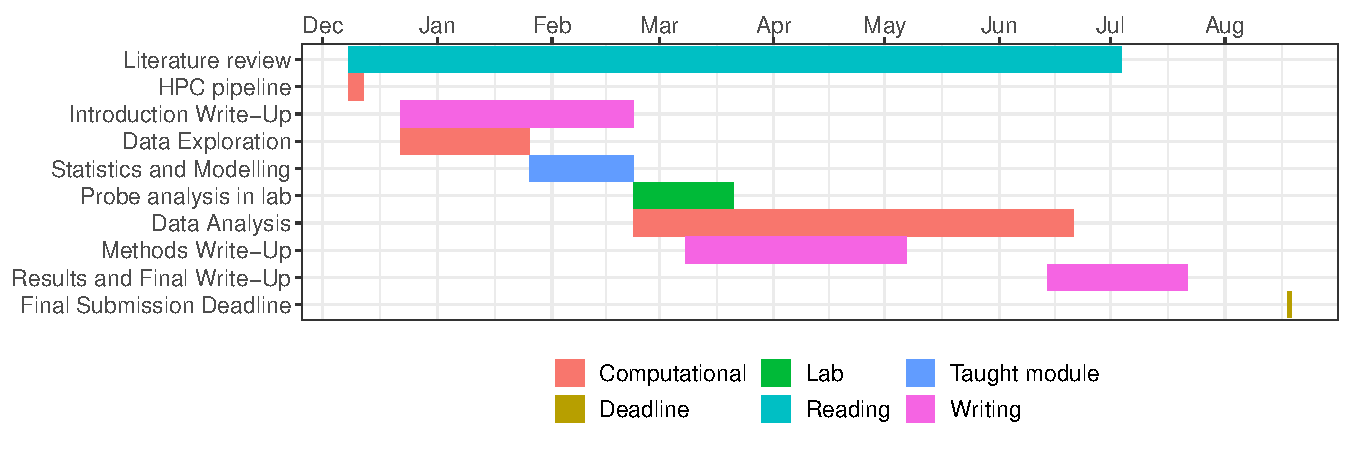
\includegraphics[width=1\textwidth]{GanttChart.pdf}
	\caption{Proposed Project Timeline}
\end{figure}

\begin{table}[h!]
	\small
	\begin{tabular} {| l | c | l |}  \hline
		\textbf{Budgeted Item} & \textbf{Cost} & \textbf{Reasoning} \\ \hline
		Herptofauna Workers Meeting 2020 & £250 & Herpetological conference cost and accommodation \\ \hline
		qPCR Reagents & £220 & To perform MiSeq runs in the laboratory \\ \hline
		Laptop Adaptor & £30 & To enable me to use USB sticks, HDMI etc. with my laptop \\ \hline
		\textbf{Total} & £500  & - \\ \hline
	\end{tabular}
	\caption{Proposed Project Budget}
\end{table}

\newpage

\printbibliography

\newpage

\section{Approval}

I have seen and approved the proposal and the budget. 
\newline
\newline
\newline
\noindent Name:
\newline
\newline
\newline
\newline
Signature:
\newline
\newline
\newline
\newline
Date:

\end{document}
